
%\documentclass[11pts,a4paper,amsmath,amssymb,floatfix]{article}%{report}%{book}
\documentclass[12pts,a4paper,amsmath,amssymb,floatfix]{article}%{report}%{book}
\usepackage{graphicx,wrapfig,pdfpages}% Include figure files
%\usepackage{dcolumn,enumerate}% Align table columns on decimal point
\usepackage{enumerate,enumitem}% Align table columns on decimal point
\usepackage{bm,dpfloat}% bold math
\usepackage[pdftex,bookmarks,colorlinks=true,urlcolor=rltblue,citecolor=blue]{hyperref}
\usepackage{amsfonts,amsmath,amssymb,stmaryrd,indentfirst}
\usepackage{times,psfrag}
\usepackage{natbib}
\usepackage{color}
\usepackage{units}
\usepackage{rotating}
\usepackage{multirow}


\usepackage{pifont}
\usepackage{subfigure}
\usepackage{subeqnarray}
\usepackage{ifthen}

\usepackage{supertabular}
\usepackage{moreverb}
\usepackage{listings}
\usepackage{palatino}
%\usepackage{doi}
\usepackage{longtable}
\usepackage{float}
\usepackage{perpage}
\MakeSorted{figure}
%\usepackage{pdflscape}


%\usepackage{booktabs}
%\newcommand{\ra}[1]{\renewcommand{\arraystretch}{#1}}


\definecolor{rltblue}{rgb}{0,0,0.75}


%\usepackage{natbib}
\usepackage{fancyhdr} %%%%
\pagestyle{fancy}%%%%
% with this we ensure that the chapter and section
% headings are in lowercase
%%%%\renewcommand{\chaptermark}[1]{\markboth{#1}{}}
\renewcommand{\sectionmark}[1]{\markright{\thesection\ #1}}
\fancyhf{} %delete the current section for header and footer
\fancyhead[LE,RO]{\bfseries\thepage}
\fancyhead[LO]{\bfseries\rightmark}
\fancyhead[RE]{\bfseries\leftmark}
\renewcommand{\headrulewidth}{0.5pt}
% make space for the rule
\fancypagestyle{plain}{%
\fancyhead{} %get rid of the headers on plain pages
\renewcommand{\headrulewidth}{0pt} % and the line
}

\def\newblock{\hskip .11em plus .33em minus .07em}
\usepackage{color}

%\usepackage{makeidx}
%\makeindex

\setlength\textwidth      {16.cm}
\setlength\textheight     {22.6cm}
\setlength\oddsidemargin  {-0.3cm}
\setlength\evensidemargin {0.3cm}

\setlength\headheight{14.49998pt} 
\setlength\topmargin{0.0cm}
\setlength\headsep{1.cm}
\setlength\footskip{1.cm}
\setlength\parskip{0pt}
\setlength\parindent{0pt}


%%%
%%% Headers and Footers
\lhead[] {\text{\small{EG3521 -- Engineering Thermodynamics}}} 
\rhead[] {{\text{\small{Tutorial 03 (2014/15)}}}}
%\chead[] {\text{\small{Session 2012/13}}} 
\lfoot[]{Dr Jeff Gomes}
%\cfoot[\thepage]{\thepage}
\rfoot[\text{\small{\thepage}}]{\thepage}
\renewcommand{\headrulewidth}{0.8pt}


%%%
%%% space between lines
%%%
\renewcommand{\baselinestretch}{1.5}

\newenvironment{VarDescription}[1]%
  {\begin{list}{}{\renewcommand{\makelabel}[1]{\textbf{##1:}\hfil}%
    \settowidth{\labelwidth}{\textbf{#1:}}%
    \setlength{\leftmargin}{\labelwidth}\addtolength{\leftmargin}{\labelsep}}}%
  {\end{list}}

%%%%%%%%%%%%%%%%%%%%%%%%%%%%%%%%%%%%%%%%%%%
%%%%%%                              %%%%%%%
%%%%%%      NOTATION SECTION        %%%%%%%
%%%%%%                              %%%%%%%
%%%%%%%%%%%%%%%%%%%%%%%%%%%%%%%%%%%%%%%%%%%

% Text abbreviations.
\newcommand{\ie}{{\em{i.e., }}}
\newcommand{\eg}{{\em{e.g., }}}
\newcommand{\cf}{{\em{cf., }}}
\newcommand{\wrt}{with respect to}
\newcommand{\lhs}{left hand side}
\newcommand{\rhs}{right hand side}
% Commands definining mathematical notation.

% This is for quantities which are physically vectors.
\renewcommand{\vec}[1]{{\mbox{\boldmath$#1$}}}
% Physical rank 2 tensors
\newcommand{\tensor}[1]{\overline{\overline{#1}}}
% This is for vectors formed of the value of a quantity at each node.
\newcommand{\dvec}[1]{\underline{#1}}
% This is for matrices in the discrete system.
\newcommand{\mat}[1]{\mathrm{#1}}


\DeclareMathOperator{\sgn}{sgn}
\newtheorem{thm}{Theorem}[section]
\newtheorem{lemma}[thm]{Lemma}

%\newcommand\qed{\hfill\mbox{$\Box$}}
\newcommand{\re}{{\mathrm{I}\hspace{-0.2em}\mathrm{R}}}
\newcommand{\inner}[2]{\langle#1,#2\rangle}
\renewcommand\leq{\leqslant}
\renewcommand\geq{\geqslant}
\renewcommand\le{\leqslant}
\renewcommand\ge{\geqslant}
\renewcommand\epsilon{\varepsilon}
\newcommand\eps{\varepsilon}
\renewcommand\phi{\varphi}
\newcommand{\bmF}{\vec{F}}
\newcommand{\bmphi}{\vec{\phi}}
\newcommand{\bmn}{\vec{n}}
\newcommand{\bmns}{{\textrm{\scriptsize{\boldmath $n$}}}}
\newcommand{\bmi}{\vec{i}}
\newcommand{\bmj}{\vec{j}}
\newcommand{\bmk}{\vec{k}}
\newcommand{\bmx}{\vec{x}}
\newcommand{\bmu}{\vec{u}}
\newcommand{\bmv}{\vec{v}}
\newcommand{\bmr}{\vec{r}}
\newcommand{\bma}{\vec{a}}
\newcommand{\bmg}{\vec{g}}
\newcommand{\bmU}{\vec{U}}
\newcommand{\bmI}{\vec{I}}
\newcommand{\bmq}{\vec{q}}
\newcommand{\bmT}{\vec{T}}
\newcommand{\bmM}{\vec{M}}
\newcommand{\bmtau}{\vec{\tau}}
\newcommand{\bmOmega}{\vec{\Omega}}
\newcommand{\pp}{\partial}
\newcommand{\kaptens}{\tensor{\kappa}}
\newcommand{\tautens}{\tensor{\tau}}
\newcommand{\sigtens}{\tensor{\sigma}}
\newcommand{\etens}{\tensor{\dot\epsilon}}
\newcommand{\ktens}{\tensor{k}}
\newcommand{\half}{{\textstyle \frac{1}{2}}}
\newcommand{\tote}{E}
\newcommand{\inte}{e}
\newcommand{\strt}{\dot\epsilon}
\newcommand{\modu}{|\bmu|}
% Derivatives
\renewcommand{\d}{\mathrm{d}}
\newcommand{\D}{\mathrm{D}}
\newcommand{\ddx}[2][x]{\frac{\d#2}{\d#1}}
\newcommand{\ddxx}[2][x]{\frac{\d^2#2}{\d#1^2}}
\newcommand{\ddt}[2][t]{\frac{\d#2}{\d#1}}
\newcommand{\ddtt}[2][t]{\frac{\d^2#2}{\d#1^2}}
\newcommand{\ppx}[2][x]{\frac{\partial#2}{\partial#1}}
\newcommand{\ppxx}[2][x]{\frac{\partial^2#2}{\partial#1^2}}
\newcommand{\ppt}[2][t]{\frac{\partial#2}{\partial#1}}
\newcommand{\pptt}[2][t]{\frac{\partial^2#2}{\partial#1^2}}
\newcommand{\DDx}[2][x]{\frac{\D#2}{\D#1}}
\newcommand{\DDxx}[2][x]{\frac{\D^2#2}{\D#1^2}}
\newcommand{\DDt}[2][t]{\frac{\D#2}{\D#1}}
\newcommand{\DDtt}[2][t]{\frac{\D^2#2}{\D#1^2}}
% Norms
\newcommand{\Ltwo}{\ensuremath{L_2} }
% Basis functions
\newcommand{\Qone}{\ensuremath{Q_1} }
\newcommand{\Qtwo}{\ensuremath{Q_2} }
\newcommand{\Qthree}{\ensuremath{Q_3} }
\newcommand{\QN}{\ensuremath{Q_N} }
\newcommand{\Pzero}{\ensuremath{P_0} }
\newcommand{\Pone}{\ensuremath{P_1} }
\newcommand{\Ptwo}{\ensuremath{P_2} }
\newcommand{\Pthree}{\ensuremath{P_3} }
\newcommand{\PN}{\ensuremath{P_N} }
\newcommand{\Poo}{\ensuremath{P_1P_1} }
\newcommand{\PoDGPt}{\ensuremath{P_{-1}P_2} }

\newcommand{\metric}{\tensor{M}}
\newcommand{\configureflag}[1]{\texttt{#1}}

% Units
\newcommand{\m}[1][]{\unit[#1]{m}}
\newcommand{\km}[1][]{\unit[#1]{km}}
\newcommand{\s}[1][]{\unit[#1]{s}}
\newcommand{\invs}[1][]{\unit[#1]{s}\ensuremath{^{-1}}}
\newcommand{\ms}[1][]{\unit[#1]{m\ensuremath{\,}s\ensuremath{^{-1}}}}
\newcommand{\mss}[1][]{\unit[#1]{m\ensuremath{\,}s\ensuremath{^{-2}}}}
\newcommand{\K}[1][]{\unit[#1]{K}}
\newcommand{\PSU}[1][]{\unit[#1]{PSU}}
\newcommand{\Pa}[1][]{\unit[#1]{Pa}}
\newcommand{\kg}[1][]{\unit[#1]{kg}}
\newcommand{\rads}[1][]{\unit[#1]{rad\ensuremath{\,}s\ensuremath{^{-1}}}}
\newcommand{\kgmm}[1][]{\unit[#1]{kg\ensuremath{\,}m\ensuremath{^{-2}}}}
\newcommand{\kgmmm}[1][]{\unit[#1]{kg\ensuremath{\,}m\ensuremath{^{-3}}}}
\newcommand{\Nmm}[1][]{\unit[#1]{N\ensuremath{\,}m\ensuremath{^{-2}}}}

% Dimensionless numbers
\newcommand{\dimensionless}[1]{\mathrm{#1}}
\renewcommand{\Re}{\dimensionless{Re}}
\newcommand{\Ro}{\dimensionless{Ro}}
\newcommand{\Fr}{\dimensionless{Fr}}
\newcommand{\Bu}{\dimensionless{Bu}}
\newcommand{\Ri}{\dimensionless{Ri}}
\renewcommand{\Pr}{\dimensionless{Pr}}
\newcommand{\Pe}{\dimensionless{Pe}}
\newcommand{\Ek}{\dimensionless{Ek}}
\newcommand{\Gr}{\dimensionless{Gr}}
\newcommand{\Ra}{\dimensionless{Ra}}
\newcommand{\Sh}{\dimensionless{Sh}}
\newcommand{\Sc}{\dimensionless{Sc}}


% Journals
\newcommand{\IJHMT}{{\it International Journal of Heat and Mass Transfer}}
\newcommand{\NED}{{\it Nuclear Engineering and Design}}
\newcommand{\ICHMT}{{\it International Communications in Heat and Mass Transfer}}
\newcommand{\NET}{{\it Nuclear Engineering and Technology}}
\newcommand{\HT}{{\it Heat Transfer}}   
\newcommand{\IJHT}{{\it International Journal for Heat Transfer}}

\newcommand{\frc}{\displaystyle\frac}

\newlist{ExList}{enumerate}{1}
\setlist[ExList,1]{label={\bf Example 1.} {\bf \arabic*}}

\newlist{ProbList}{enumerate}{1}
\setlist[ProbList,1]{label={\bf Problem 1.} {\bf \arabic*}}

%%%%%%%%%%%%%%%%%%%%%%%%%%%%%%%%%%%%%%%%%%%
%%%%%%                              %%%%%%%
%%%%%% END OF THE NOTATION SECTION  %%%%%%%
%%%%%%                              %%%%%%%
%%%%%%%%%%%%%%%%%%%%%%%%%%%%%%%%%%%%%%%%%%%


% Cause numbering of subsubsections. 
%\setcounter{secnumdepth}{8}
%\setcounter{tocdepth}{8}

\setcounter{secnumdepth}{4}%
\setcounter{tocdepth}{4}%


\begin{document}



\begin{enumerate}[label=\bfseries Problem \arabic*]

%%%
%%% Lecture Notes
%%%
\item\label{Tut03:CarnotEfficiency} Steam (dry and saturated) is supplied by the boiler at 15 bar and the condenser pressure is 0.4 bar. Calculate the Carnot and Rankine efficiencies of the cycle. Neglect the pump work.


%%%
%%% Lecture Notes
%%%
\item\label{Tut03:SimpleSteamPowerPlant}The table below represents the steps of an idealised steam power plant:
    \begin{center}
     \begin{tabular}{||c | c | c | c | c | c ||}
      \hline\hline
       {\bf Step} & {\bf Location}       & {\bf Pressure}  & {\bf Temperature}     & {\bf Quality /}  &{\bf Velocity}    \\
                  &                      & {\bf (bar)}     &{\bf$\left(^{\circ}\text{C}\right)$}& {\bf State} & {\bf m/s} \\
      \hline\hline
          1       & Inlet to turbine     &   60            &   380                 &  --              &       --         \\
      \hline
          2       & Exit from turbine and&   0.1           &    --                 & 0.9              &  200             \\
                  & inlet to condenser   &                 &                       &                  &                  \\ 
      \hline
          3       & Exit from condenser and&  0.09         &  --                   & Saturated        &  --              \\
                  & inlet to pump        &                 &                       & Liquid           &   --             \\
      \hline
          4       & Exit from pump and   &  100            &   --                  &     --           &   --             \\
                  & inlet to boiler      &                 &                       &                  &                  \\
      \hline 
          5       & Exit from boiler     &  80             &  440                  &      --          &    --            \\
           \hline\hline
     \end{tabular}
    \end{center}
    Assume that the steam mass flow rate leaving the boiler is 10$^{4}$ kg.h$^{-1}$. Sketch the cycle numbering each stage. Calculate:
      \begin{enumerate} 
         \item Specific enthalpies of all streams;
         \item Power output of the turbine;
         \item Heat transfer per hour in the boiler and condenser;
         \item Mass rate of cooling water circulated (kg/h) in the condenser assuming inlet and outlet fluid temperatures from the condenser of 20$^{\circ}$C and 30$^{\circ}$C. Assume the heat capacity at constant pressure of the cooling water $\left(C_{p}\right)$ is 4.18 $\frc{\text{kJ}}{\text{kg.}^{\circ}\text{C}}$;
         \item Diameter of the pipe connecting the turbine with the condenser;
         \item Sketch the $Ts$ diagram, indicating each step of the cycle.
    \end{enumerate}

%%%
%%% Lecture Notes
%%%
\item\label{Tut03:ReheatRankine}In the secondary cooling circuit of a nuclear power plant, the steam generator (boiler / reheater) produces superheated steam (SHS, Fig.~\ref{Fig_Tut03:ReheatRankine}) and is connected to two turbines operating as a reheat Rankine cycle. Isentropic efficiencies of the first $\left(\eta_{\text{T1}}\right)$ and second $\left(\eta_{\text{T2}}\right)$ turbines and boiler feed pump $\left(\eta_{\text{P}}\right)$ are 84$\%$, 80$\%$ and 61$\%$ respectively. Determine {\it (a)-(j)} in Table~\ref{Table_Tut03:ReheatRankine}. Sketch the $Ts$ diagram of the cycle.

         \begin{table}[h]
       \begin{center}
         \begin{tabular}{c | c c c c c  }
           \hline
           {\bf Stage} & $P$    & $T$             &  State            & $h$                 & $s$                      \\
                       & (bar)  & ($^{\circ}$C)    &                   & (kJ.kg$^{-1}$)       & (kJ.(kg.K)$^{-1}$)        \\
           \hline
            {\bf 1 }   & 40         & 370         & SHS               & {\bf (a)}           & {\bf (b)}                 \\
            {\bf 2 }   &  --        &  --         & {\bf (c)}         & --                  &   --                      \\
            {\bf 3 }   & 7          & 370         & SHS               & {\bf (d)}           & {\bf (e)}                 \\
            {\bf 4 }   & 0.10       & --          &     --            & --                   & --                      \\
            {\bf 5 }   & 0.10       & --          &   {\bf (f)}       & {\bf (g)}           & {\bf (h)}                 \\
            {\bf 6 }   & 40         & --          &   {\bf (i)}       & {\bf (j)}           & --                       \\
           \hline
         \end{tabular}
          \caption{\ref{Tut03:ReheatRankine}.}\label{Table_Tut03:ReheatRankine}
        \end{center}
         \end{table} 
    
           \begin{figure}[h]
         \begin{center}
            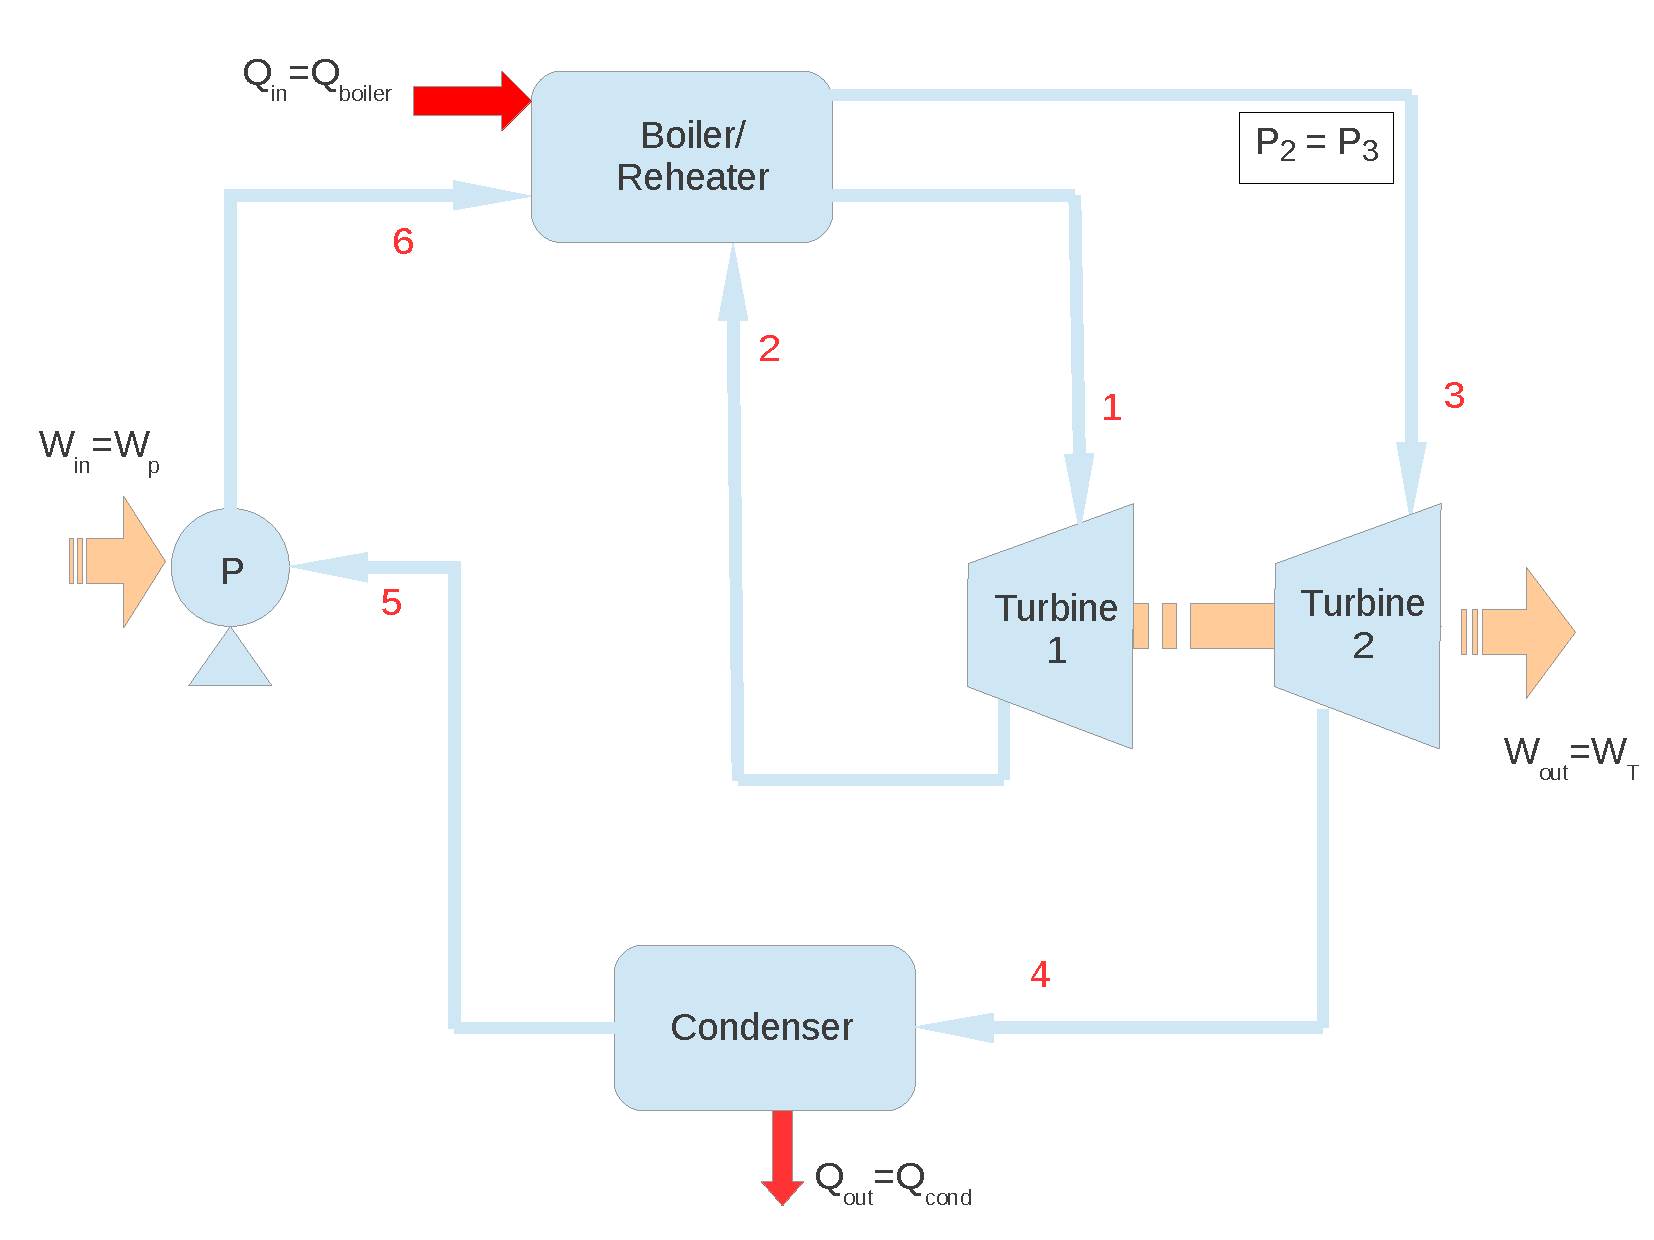
\includegraphics[width=9.5cm,clip]{./Pics/Exam_Reheat_Rankine_Cycle}
          \caption{\ref{Tut03:ReheatRankine}}\label{Fig_Tut03:ReheatRankine}
         \end{center}
           \end{figure}

%%%
%%%
%%%
\item \label{Problem_02:01}A Carnot engine with water/steam (1 kg/s) as the working fluid operates on the cycle shown in Fig. \ref{PVTSDiags}. For $T_{1}=475\;K$ and $T_{2}=300\;K$, determine: (a) pressures at states 1, 2, 3, and 4; (b) quality $x^{\text{vapour}}$ at states 2 and 3; (c) rate of heat addition; (d) rate of heat rejection; (e) mechanical power for each of the four steps; (f) thermal efficiency $\left(\eta\right)$ of the cycle.
   \begin{figure}[h]
    \begin{center}
     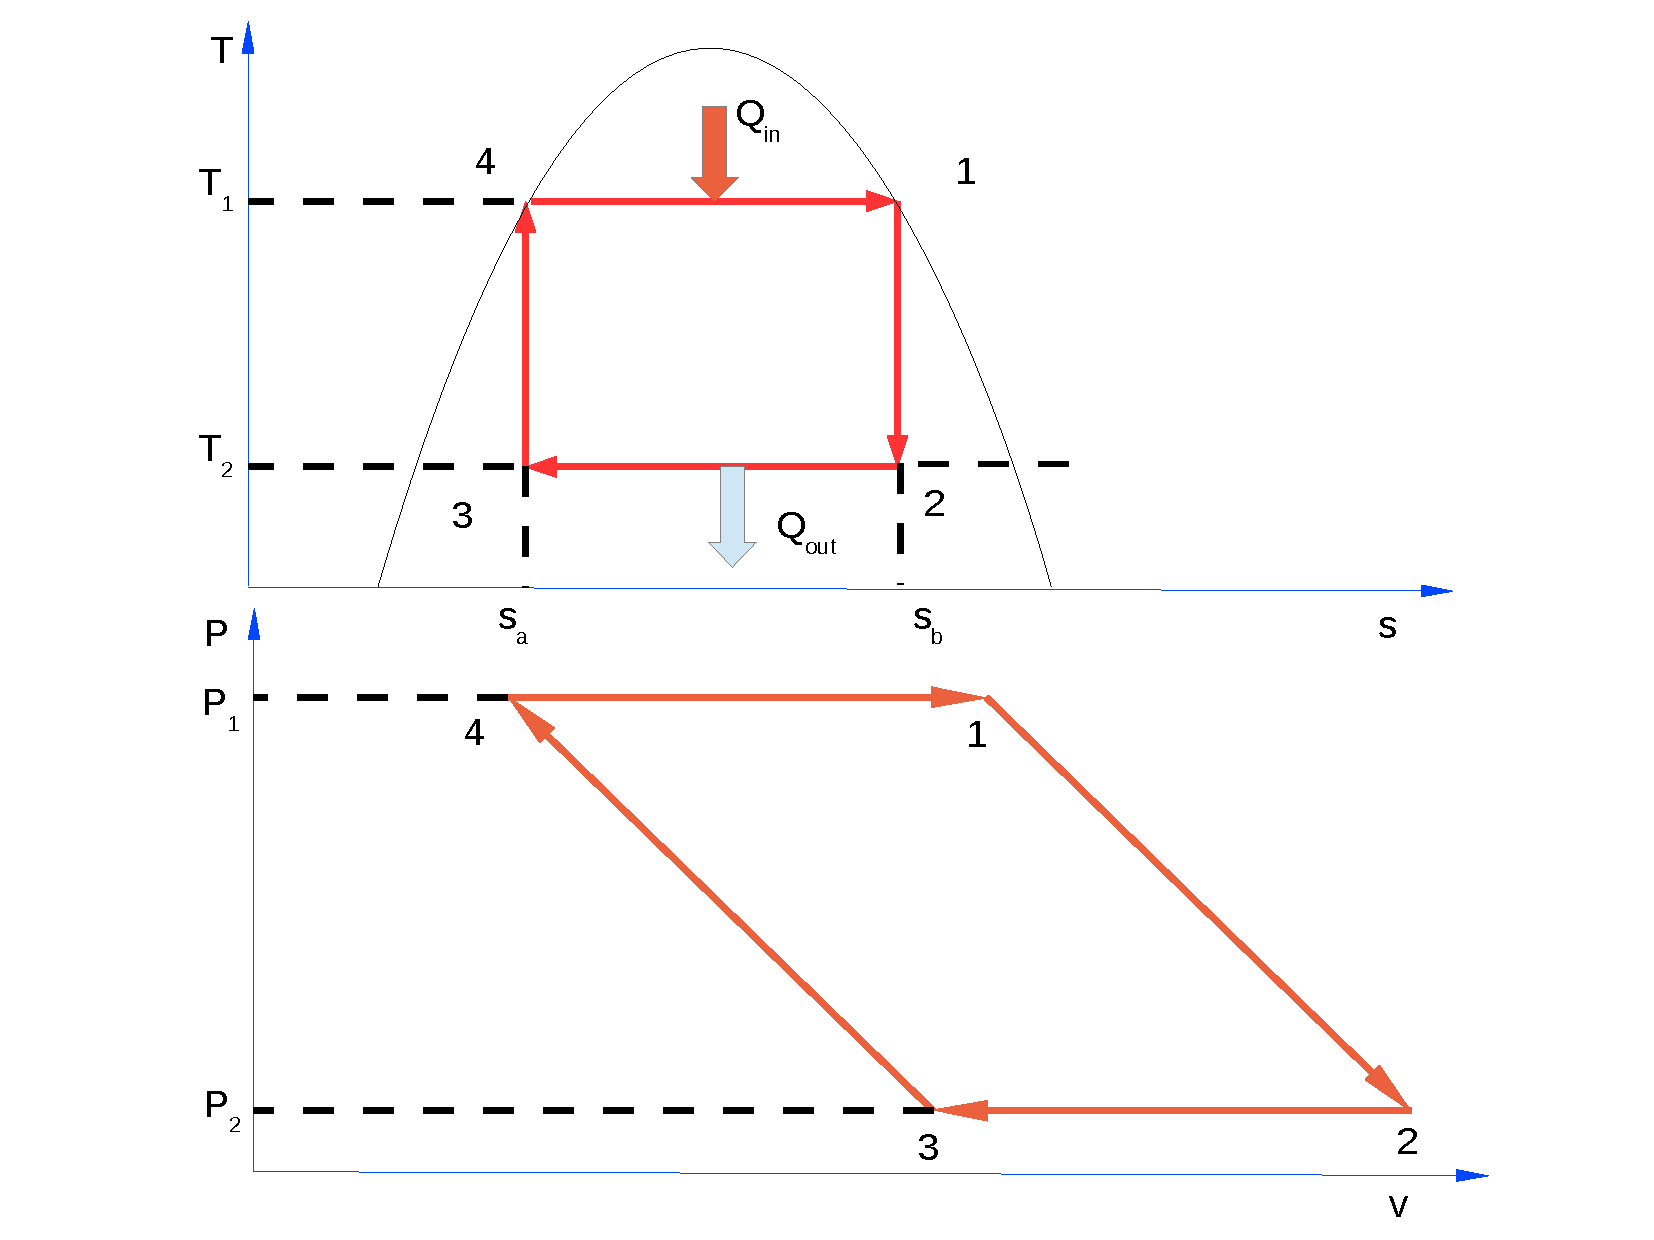
\includegraphics[width=12.cm,clip]{./Pics/Carnot_PV_TS}
    \end{center}
    \caption{Ts and Pv diagrams for Carnot cycle (\ref{Problem_02:01}).}\label{PVTSDiags}
   \end{figure}    


%%%
%%% Problem 8.6 (Saphiro)
%%%
\item\label{Tut03:Saphiro8.6} Water is the working fluid in an ideal Rankine cycle. Saturated vapour enters the turbine at 16 MPa, and the condenser pressure is 8 kPa. The mass flow rate of steam entering in the turbine is 120 kg/s. Calculate:
\begin{enumerate}
\item the net power developed (in MW);
\item rate of heat transfer to the steam passing through the boiler (in MW);
\item thermal efficiency;
\item mass flow rate of the condenser cooling water (in kg/s), if the cooling water undergoes a temperature increase of 18$^{o}$C with negligible pressure change in passing through the condenser.
\end{enumerate} 



%%%
%%% Example 12.25 (Rajput)
%%%
\item\label{P:example12_25} A steam power plant operates with with regenerative and reheat arrangement cycles. Steam is supplied to the H.P. turbine (Fig. \ref{example12_25}a) at 80 bar and 470$^{o}$C.  For feed heating, a part of steam is extracted at 7 bar and remainder of the steam is reheated to 350$^{o}$C in a reheater and then expanded in L.P. turbine down to 0.035 bar. Determine: (a) amount of steam bled-off for feed heating; (b) amount of steam supplied to L.P. turbine; (c) heat supplied to the boiler and reheater; (d) cycle efficiency, and (e) power developed by the system. The steam supplied by the boiler is 50 kg/s.
   \begin{figure}[h]
    \begin{center}
    \vbox{
     \hbox{\hspace{1cm}
      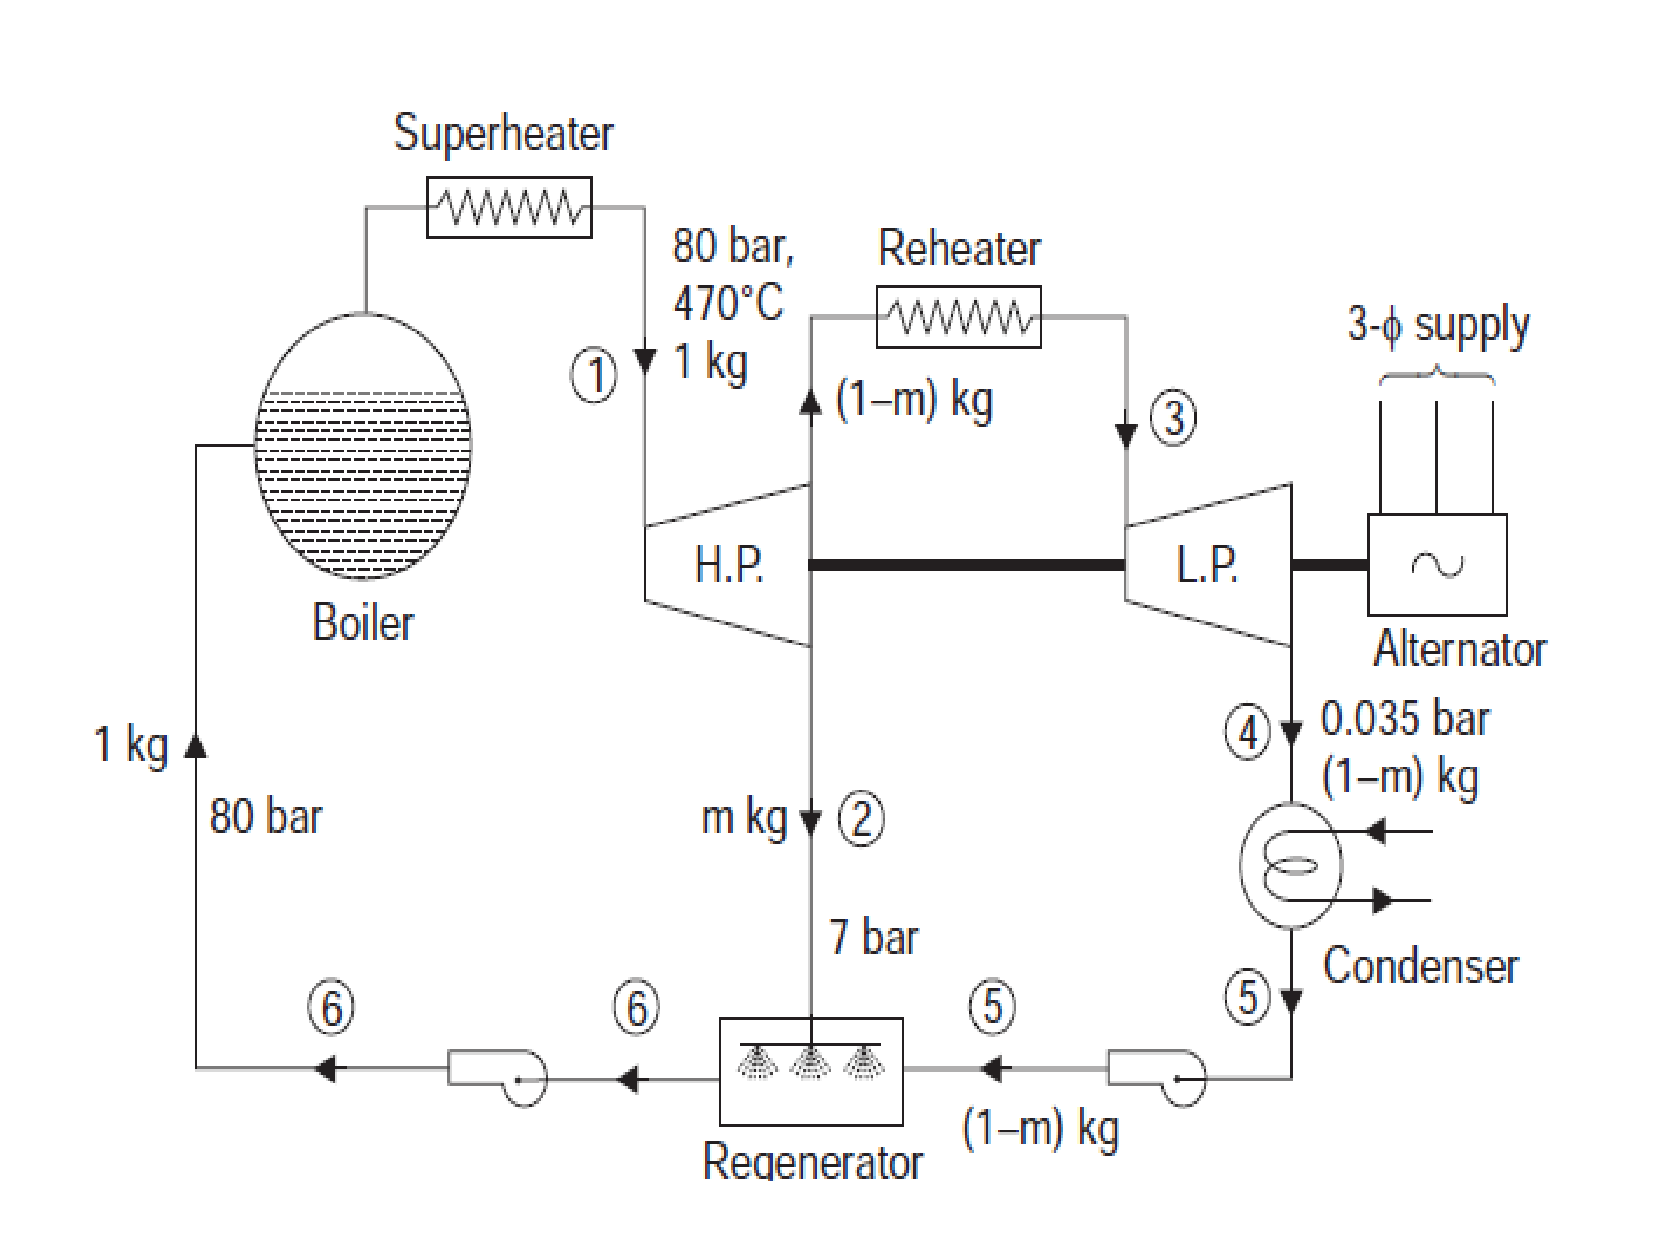
\includegraphics[width=12.cm,clip]{./Pics/Exemple12_25a_Rajput}}
     \hbox{\hspace{7.5cm}(a)}
     \hbox{\hspace{1.cm}
      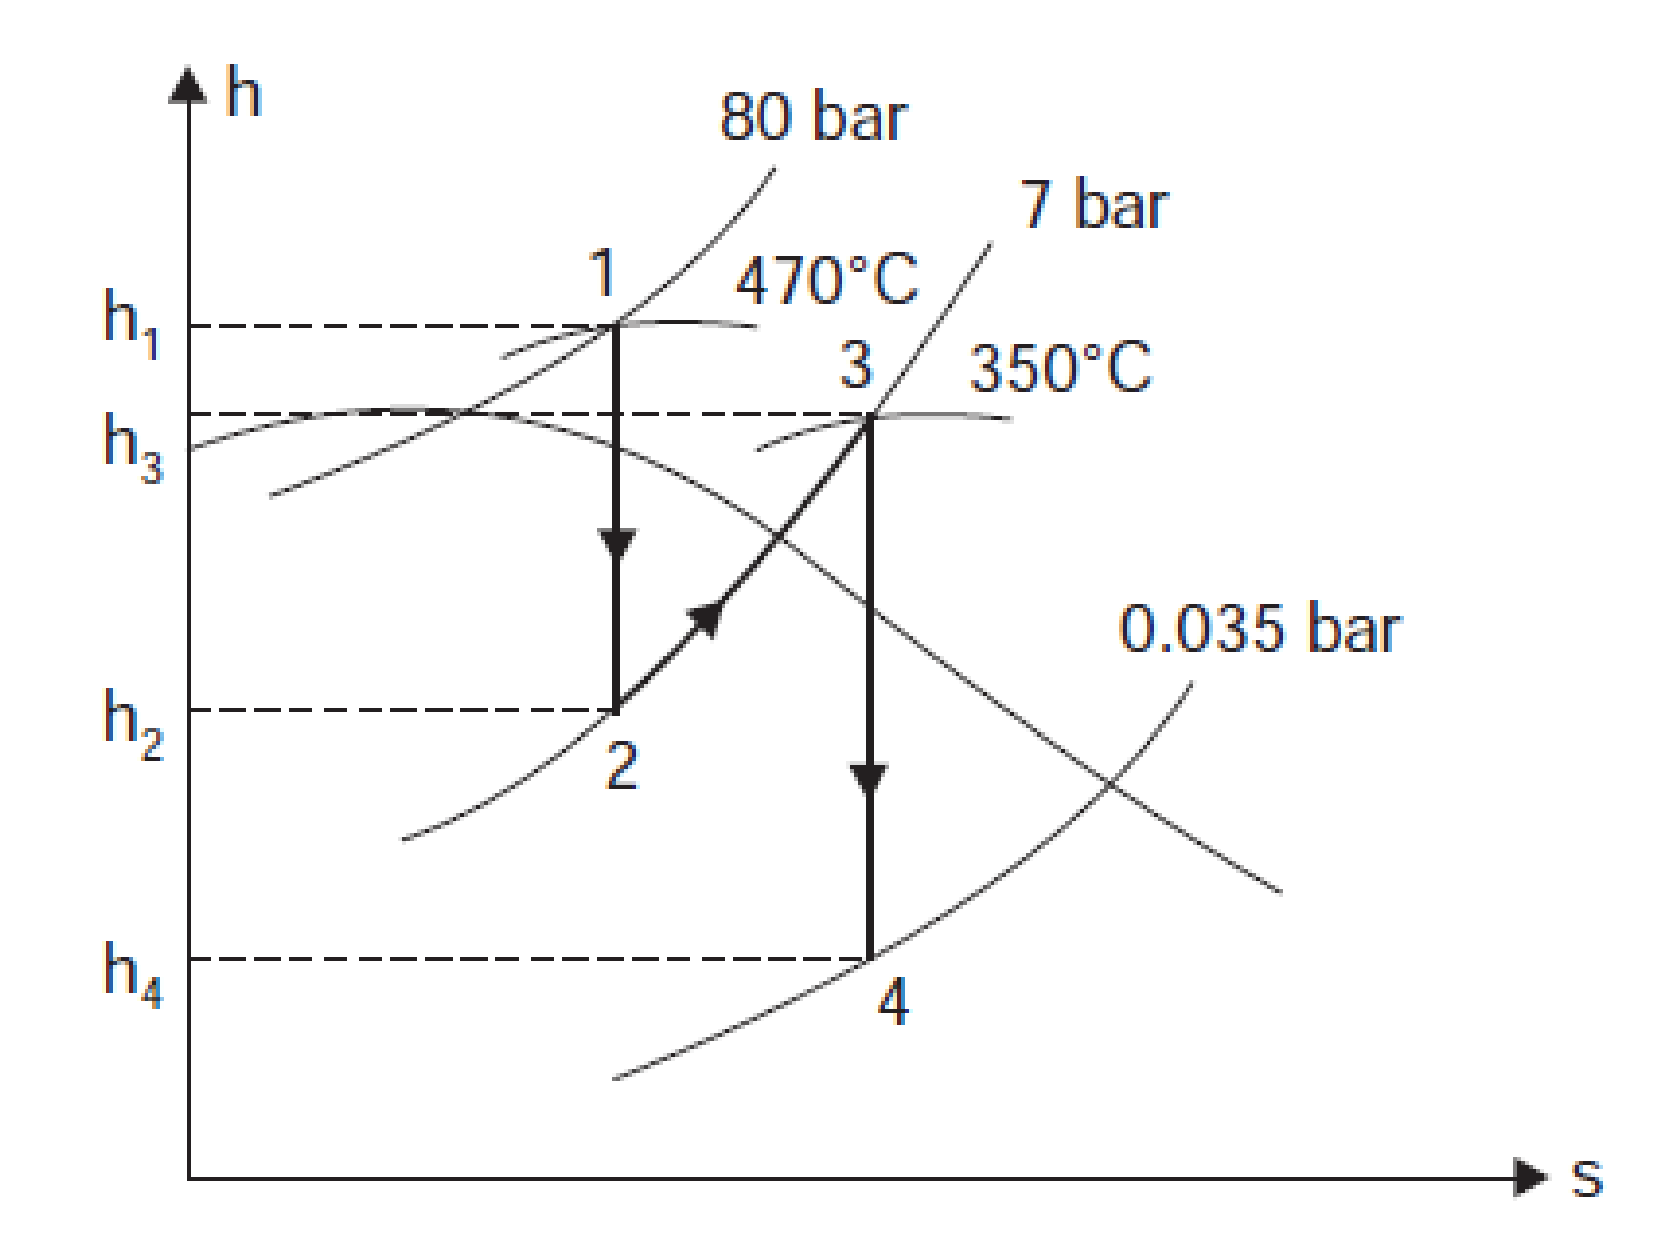
\includegraphics[width=12.cm,clip]{./Pics/Exemple12_25b_Rajput}
      }
     \hbox{\hspace{7.5cm}(b)}}
     \caption{ (a) Schematics and (b) $hs$ diagram of a steam power cycle (\ref{P:example12_25}).}
     \label{example12_25}
     \end{center}
   \end{figure}
 


%%%
%%% Problem 8.9 (SM&VN). \ref{example8_9})
%%%
\item \label{P:example8_9}Steam power plant operating on a regenerative cycle, includes just one feedwater heater. Steam enters the turbine at 4500 kPa and 773.15 K and exhausts at 20 kPa. Steam for the feedwater heater is extracted from the turbine at 350 kPa, and in condensing raises the temperature of the feedwater to within 6 K of its condensation temperature at 350 kPa. If the turbine and pump efficiencies are both 0.78, what is the thermal efficiency of the cycle and what fraction of the steam entering the turbine is extracted for the feedwater heater? Assume that the enthalpy of the water fed into the boiler $\left(h_{i}\right)$ is given by
\begin{displaymath}
h_{i} = h_{\text{liquid}}^{\text{sat}} + v_{\text{liquid}}^{\text{sat}}\left(1-\beta T_{i}\right)\left(P_{i}-P^{\text{sat}}\right) 
\end{displaymath} 
where $v$ is the specific volume and $\beta=\frc{1}{v}\left(\frc{\partial v}{\partial T}\right)_{P}$ is the volume expansivity of the water.

\end{enumerate}



\clearpage

%{
%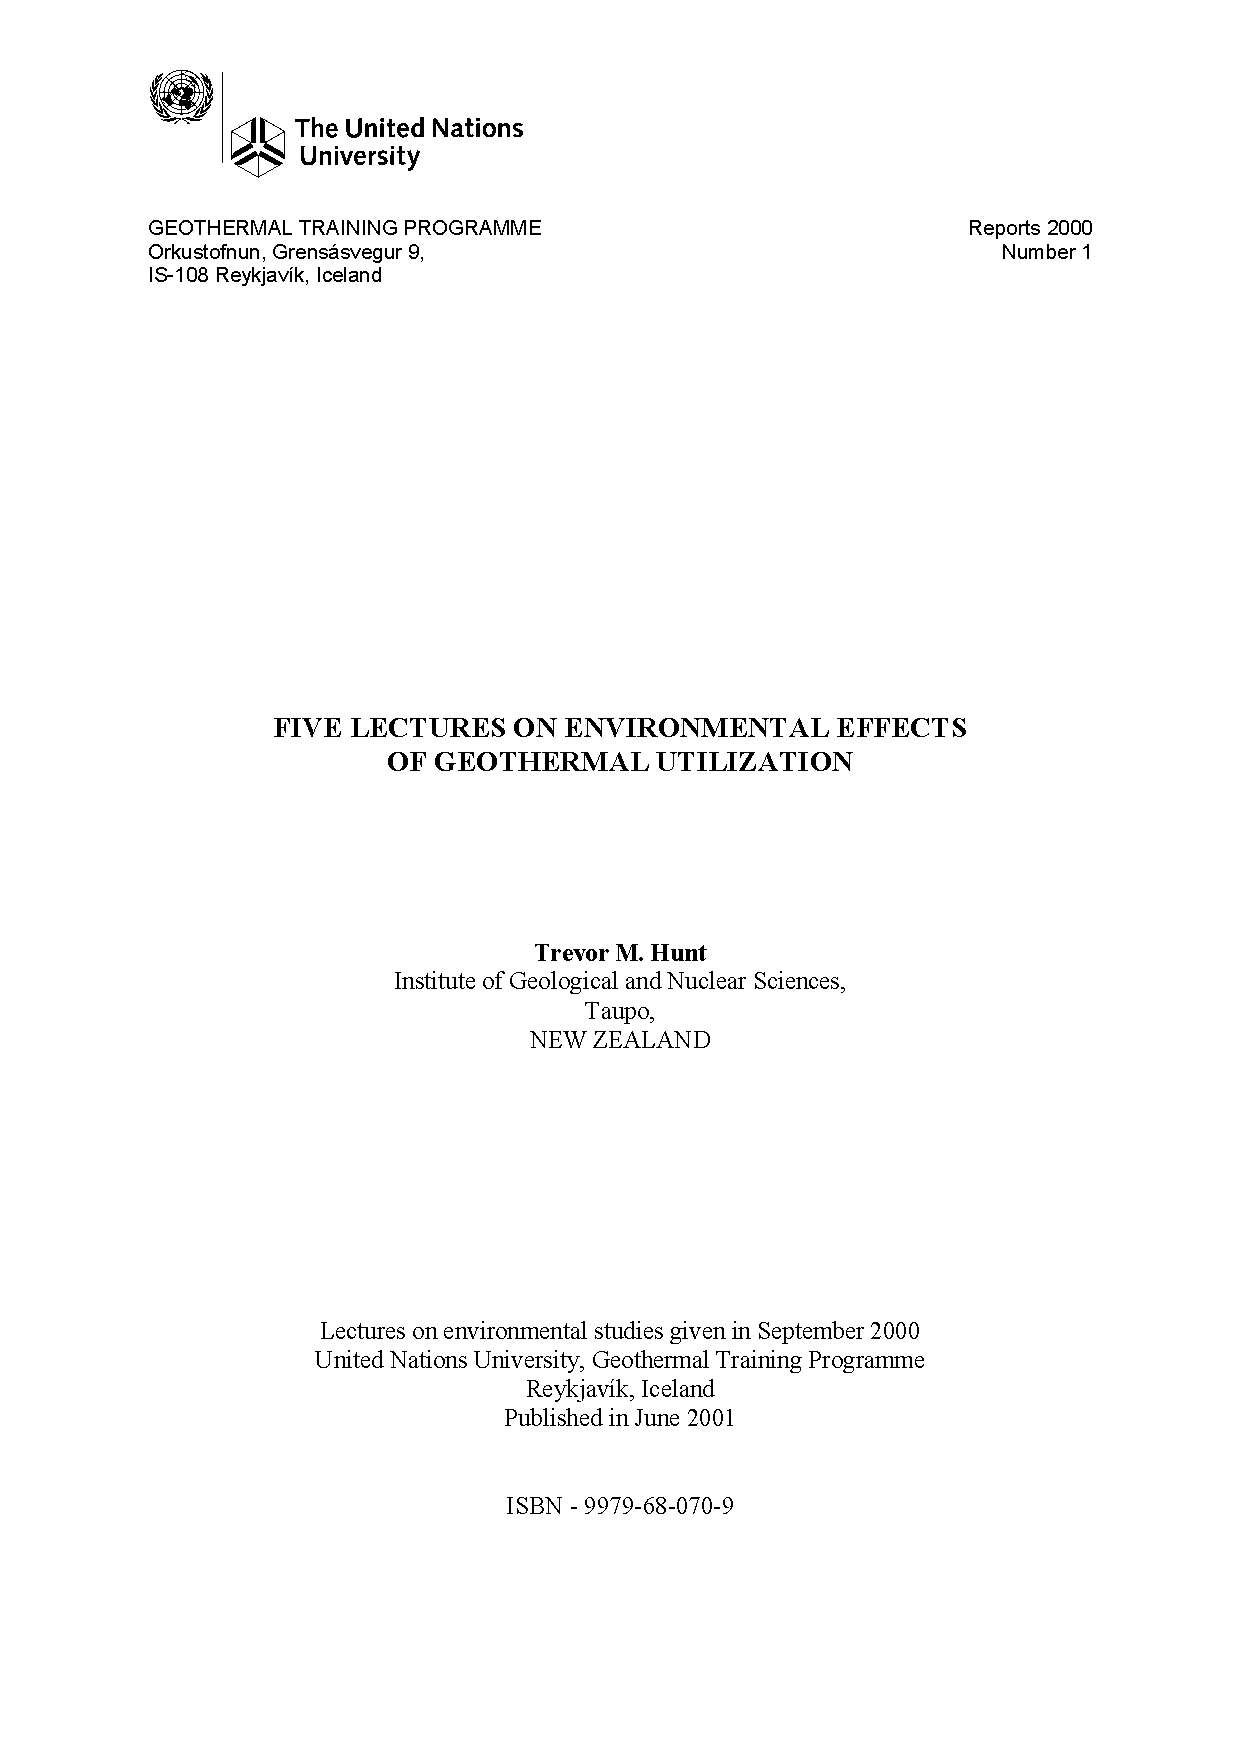
\includepdf[pages=-,fitpaper, angle=0]{./HuntSelect.pdf}
%}

\end{document}
